\documentclass[12pt,a4paper]{article}
\usepackage[utf8]{inputenc}
\usepackage[spanish]{babel}
\usepackage{amsmath}
\usepackage{amsfonts}
\usepackage{amssymb}
\usepackage{graphicx}
\author{Manuel González González}
\title{Práctica 8: Red Autoorganizada}
\begin{document}
\maketitle

\section*{Ejercicio 3}

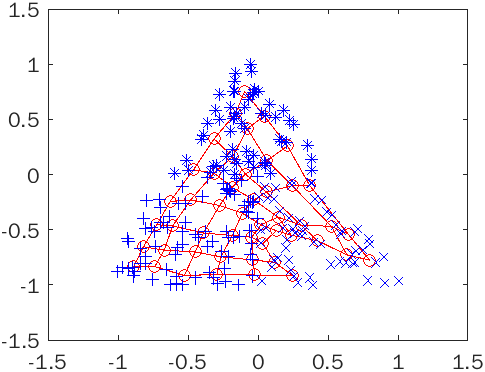
\includegraphics[scale=1]{it1.png}
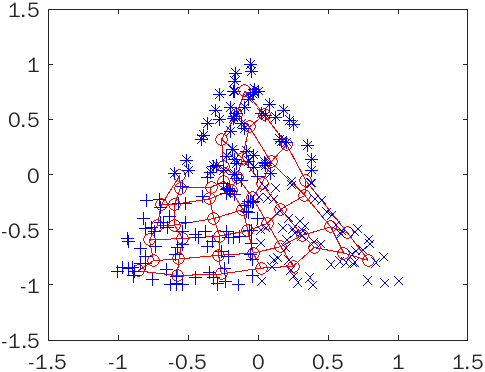
\includegraphics[scale=1]{it2.png}
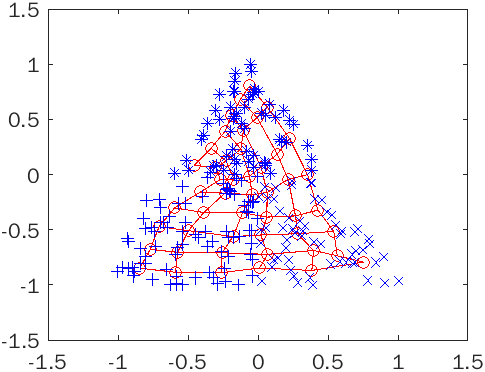
\includegraphics[scale=1]{it3.png}

\subsection*{a)}

El resultado no es el mismo siempre. Esto se debe a la aleatoriedad puesta en la matriz principal de pesos y en la aleatoriedad de los índices de los datos, ya que en cada ejecución el orden en el que ganan las neuronas y con cuánto peso lo hacen va a cambiar el resultado final.


\subsection*{b)}

Cubren bien la forma objetivo ya que cada neurona ganadora modifica a su vez a las vecinas, haciendo que no se quede ninguna muerta y ayudando a suavizar el aprendizaje, lo cual evita que en el recubrimiento queden zonas muy dispares con menos representación de la que cabría esperar.


\end{document}